\documentclass{standalone}

\usepackage{pgfplots,tikz,amsmath}
\begin{document}
        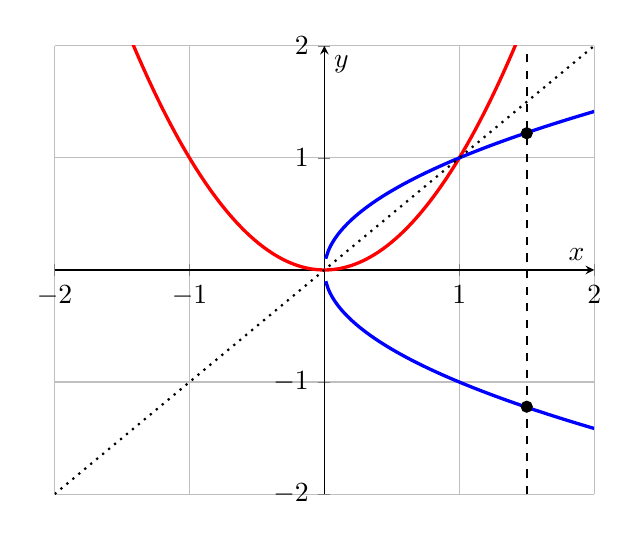
\begin{tikzpicture}
            \begin{axis}[axis lines=center, xlabel={$x$}, ylabel={$y$}, domain=-2:2,
                ymin=-2, ymax=2, xmin=-2, xmax=2, grid]
                \addplot[smooth, very thick, red, samples=150] {x^2};
                \addplot[smooth, very thick, blue, samples=200] {sqrt(x)};
                \addplot[smooth, very thick, blue, samples=200] {-sqrt(x)};
                \addplot[smooth, black, dotted, thick] {x};
                \draw[black, dashed, thick] (axis cs:1.5,-2) -- (axis cs:1.5,2);
                \draw[fill=black] (axis cs:1.5,1.22) circle(0.07cm);
                \draw[fill=black] (axis cs:1.5,-1.22) circle(0.07cm);
            \end{axis}
        \end{tikzpicture}
        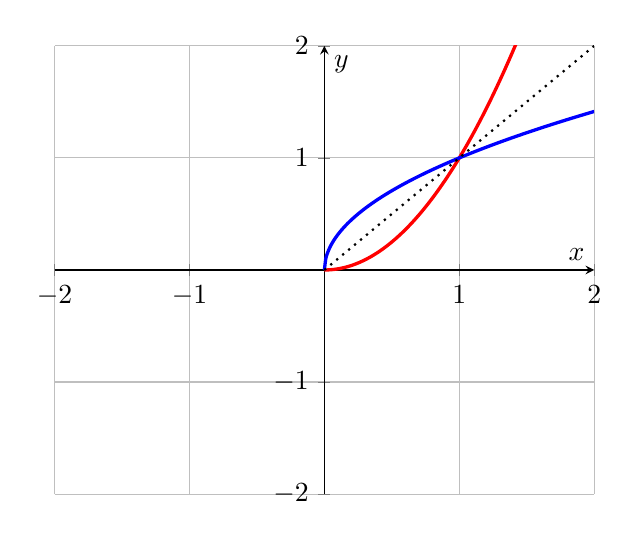
\begin{tikzpicture}
            \begin{axis}[axis lines=center, xlabel={$x$}, ylabel={$y$}, domain=0:2,
                ymin=-2, ymax=2, xmin=-2, xmax=2, grid]
                \addplot[smooth, very thick, red, samples=200] {x^2};
                \addplot[smooth, very thick, blue, samples=200] {sqrt(x)};
                \addplot[smooth, black, dotted, thick] {x};
            \end{axis}
        \end{tikzpicture}
\end{document}
